\documentclass[acmsmall,anonymous]{acmart}

% Packages {{{
\usepackage{amsmath}
\usepackage{amssymb}
\usepackage{tikz}
\usetikzlibrary{calc}
\usetikzlibrary{graphs}
\usetikzlibrary{cd}
\usepackage{bussproofs}
% }}}

% Macros {{{

\newcommand{\kw}[1]{\ensuremath{ \textsf{#1} }}
\newcommand{\ifr}[1]{\ [{#1}]\ }
\newcommand{\ifrw}[2]{\ [{#1}]_{#2}\ }
\newcommand{\alt}{\ |\ }

\newcommand{\EC}{\kw{C}}

% Moves
\newcommand{\mcall}[3]{\kw{#1}({#2})@{#3}}
\newcommand{\pcall}[3]{%
  \underline{\mcall{#1}{#2}{#3}}%
}
\newcommand{\mret}[2]{{#1}@{#2}}
\newcommand{\pret}[2]{%
  \underline{\mret{#1}{#2}}%
}

% Pointers for justified sequences %{{{

% Parameters
\newcommand{\pshift}{1.6ex}
\newcommand{\pcdist}{2.5}
\newcommand{\pcangle}{60}

% Pointer hook
\newcommand{\ph}[1]{%
  \tikz[remember picture]{\coordinate (#1);}}

% Pointer to
\newcommand{\pt}[1]}}

% }}}

% Various parameters {{{
\bibliographystyle{ACM-Reference-Format}
\citestyle{acmauthoryear}
%}}}

\begin{document}

\title{Lightweight Compositional Compcert}

\author{J\'er\'emie Koenig}
\affiliation{
  \department{Computer Science}
  \institution{Yale University}
}
\email{jeremie.koenig@yale.edu}

\begin{abstract}
A simple game semantics based on standard Hyland-Ong games
is defined for the Compcert Clight and Asm languages,
along with appropriate notions of simulation and linking,
and the correctness theorem of CompCertX \citep{popl15}
is generalized to that setting,
turning it into a compositional compiler
similar to Compositional Compcert \citep{compcomp}.
This is achieved through
a correspondance with the original operational semantics +
Compcert KLR +
oracle construction +
some theorems about games.
\end{abstract}

\maketitle

\section{Introduction} %{{{

Problem:
compositional compilation.
System code:
link compiled C code with less well-behaved assembly code,
interact and compose with components of different types
(hardware, networks, etc.).

Existing things limited:
Compositional Compcert only works with one type of games
and proof requires modifying Compcert pretty deep,
new techniques and lots of effort to implement,
hence hard to integrate to mainstream Compcert.

Our semantic algebra less ad-hoc and follows HO games.

Our technique allow us to prove a linking theorem for Compcert
without modifying the original proofs:
leverage the external functions interface as a hook
through which we can expose Compcert to its environment in a controlled way.
Bridge the gap with some game-theoretic algebra.

KLR/parametricity understanding of Compcert languages provides
uniform easy natural definition of refinement
that works well with the existing code,
shed new light on the construction of Compcert.

\subsection{Contributions}

A new approach for building compositional certified compilers:
\begin{itemize}
\item (first applied?) mechanized formalisation of HO games
\item Compcert KLRs
\item extend KLR to strategies, game-theoretic simulations
\item simulation reflection theorem
\item game-theoretic characterization of CompCertX's correctness theorem, from which we derive
\item a \emph{semantic} contextual refinement property
\end{itemize}

%}}}

\newpage
\section{Background} %{{{

[Idea:
Explain here briefly Compcert, HO games, KLR,
to fix notation and fill in the unfamiliar reader,
but keep it standard
so that experts can skip this part.]

\subsection{Hyland-Ong games} %{{{

Games, arenas, etc.

%}}}

\subsection{Kripke logical relations} %{{{

%}}}

\subsection{The Compcert certified compiler} %{{{

Basics.

Memory model \citep{compcertmmv2}.

External call interface, CertiKOS, CompCertX \citep{popl15}.

Events.

%}}}

\subsection{Clight} %{{{

[Q: define $\rightarrow^?$,
or use $\textsf{EC} = \varnothing, \textsf{Kstop}$/parametric?]

%}}}

\subsection{Asm} %{{{

[Q: define $\rightarrow^?$,
or use $\textsf{EC} = \varnothing, \textsf{RA = Vundef}$/parametric?]

%}}}

\subsection{CompCertX and environment oracles}

%}}}

\newpage
\section{Games} %{{{

\subsection{Arenas and games} %{{{

[Probably follow \citep{gamesem99},
because we care about the distinction between $\EC$ and $!\EC$
(so \citep{gref98} not an option -- is that really true?)
but we don't care about full abstraction
(so 

%}}}

\subsection{Compcert games} %{{{

The operational semantics defined in Compcert
use the following transition relation as a parameter,
which represents the behavior of external functions.
Ignoring the global environment and event traces for now:
\[
  \kw{external\_call} :
    \kw{ident} \rightarrow
    \kw{val}^* \times \kw{mem} \rightarrow
    \mathcal{P}(\kw{val} \times \kw{mem})
\]
Given a function name,
an initial memory state,
and a list of actual parameters,
$\kw{external\_call}$ gives a set of possible final states,
each comprised of a memory state and return value.
Based on this protocol,
we define our basic Compcert game.

\begin{definition}[Elementary Compcert game]
The arena $\EC = (M_\EC, \lambda_\EC, \vdash_\EC)$
uses the following set of moves.
Moves of the form
$\mcall{f}{\vec{v}}{m} \in M_\EC^\kw{call}$
represent function calls requested by \kw{O},
while moves of the form
$\mret{v}{m'} \in M_\EC^\kw{ret}$
correspond to \kw{P}'s possible responses.
\begin{align*}
  M_\EC^\kw{call} &:=
    \{ \mcall{f}{\vec{v}}{m} :
      (f, \vec{v}, m) \in \kw{ident} \times \kw{val}^* \times \kw{mem} \} \\
  M_\EC^\kw{ret} &:=
    \{ \mret{v}{m'} :
      (v, m') \in \kw{val} \times \kw{mem} \} \\
  M_\EC &:= M_\EC^\kw{call} \cup M_\EC^\kw{ret}
\end{align*}
Accordingly, the labelling function for $\EC$ is defined as:
\[
  \lambda_\EC(e) :=
     \begin{cases}
        \kw{OQ} & \mbox{if } e \in M_\EC^\kw{call} \\
        \kw{PA} & \mbox{if } e \in M_\EC^\kw{ret} \,,
     \end{cases}
\]
and the enabling relation is defined by:
\[
  \star \ \vdash_\EC\ 
  \mcall{f}{\vec{v}}{m} \ \vdash_\EC\ 
  \mret{v}{m'} \,.
\]
\end{definition}

The game consists in a series of queries by \kw{O}
which specify a function identifier $f$,
a list of actual parameters $\vec{v}$, and
an initial memory state $m$.
\kw{P} answers each query by specifying
a return value $v$ and
a final memory state $m'$.
One possible play could be:
\[
  \mcall{\kw{f}}{\kw{Vint}(5)}{m_1}\ph{f}\ \cdot\ 
  \pt{f}\pret{\kw{Vundef}}{m_2}\ \cdot\ 
  \mcall{\kw{g}}{}{m_3}\ph{g}\ \cdot\ 
  \pt{g}\pret{\kw{Vint}(42)}{m_4}
\]
We will omit \kw{val} constructors when the type of values is clear from context:
\[
  \mcall{\kw{f}}{5}{m_1}\ph{f}\ \cdot\ 
  \pt{f}\pret{\kw{Vundef}}{m_2}\ \cdot\ 
  \mcall{\kw{g}}{}{m_3}\ph{g}\ \cdot\ 
  \pt{g}\pret{42}{m_4}
\]

The strategies for $\EC$ that we will consider
will usually be well-bracketed and innocent.
The set of such strategies corresponds exactly to
the possible Compcert external call transition relations.
Nevertheless,
as illustrated in Sec~\ref{sec:longjmp},
the ability to specify and invoke external functions
whose behavior violates these requirements
is an important feature of our work.
[Or: we don't allow repeats in $\EC$, only in $!\EC$,
so that any possible strategy for $\EC$ is innocent and well-bracketed.
Note that innocent and well-bracketed strategies for $!\EC$
are of the form $\sigma^\dagger$ where $\sigma : \EC$.
One reason to distinguish $\EC$ from $!\EC$
is that then our semantics with oracle can be expressed as
$!\EC \multimap \EC$.]

%}}}

\subsection{Open modules} %{{{

[Recast previous work in those terms:]
For a fixed behavior of external functions,
the semantics of closed modules can be
formulated as a strategy for $\EC$.
This is essentially what is done in \citep{popl15}.
Getting rid of the $\kw{external\_call}$ parameter,
a somewhat more satisfying approach is
to interpret the semantics of closed modules
as strategies for
$!\EC \multimap \EC$.
Here,
the initial move is a function call into the module,
which can then perform
an arbitrary number of external calls,
which will immediately return.
Finally,
the module answers the initial function call
with its own return move.
This is the view informally taken in \citep{osdi16},
where the memory states are instrumented with a \kw{log}
of the current interaction,
which can then be used by
a fixed $\kw{external\_call}$ predicate
to query an oracle representing the environment.
[Do more of that, explain layers etc.
Or maybe in the Related Work section?]
The work presented here goes one step further
and interprets modules as strategies for $!\EC \multimap !\EC$.
This means that
when a module calls back into the environment,
instead of returning immediately
the environment itself
can perform a nested call into the module,
and so on recursively.

The arena corresponding to these games
has 4 kinds of moves.
Schematically:
\begin{center}
  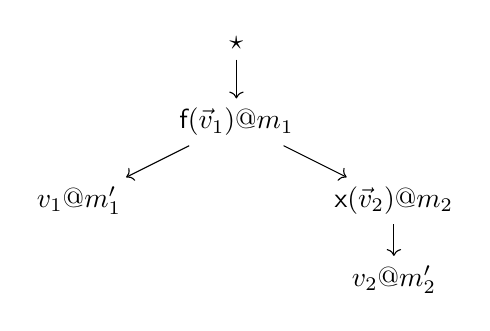
\begin{tikzpicture}
    \graph [no placement]
    {
      "$\star$" [at={(0,1)}] ->
      "$\mcall{f}{\vec{v}_1}{m_1}$" -> {
        "$\mret{v_1}{m_1'}$" [at={(-2,-1)}],
        "$\mcall{x}{\vec{v}_2}{m_2}$" [at={(+2,-1)}] ->
        "$\mret{v_2}{m_2'}$" [at={(+2,-2)}]
      }
    };
  \end{tikzpicture}
\end{center}
[Note the correspondance with Princeton core semantics.]
By convention,
in examples we name $f, g, h$
the functions exported by the module being considered,
and we name $x, y, z$
any external functions.
Moreover,
the polarity of moves makes it easy to distiguish
between the two versions of $\mcall{f}{\vec{v}}{m}$
and $\mret{v}{m'}$.
A possible interaction is:
\[
  \rule{0pt}{1.5em}
  \mcall{f}{}{m_1}\ph{f} \ \cdot\ 
  \pt{f}
    \pcall{x}{1}{m_2}\ph{x} \ \cdot\ 
    \pt{x}
      \mret{7}{m_3} \ \cdot \ 
  \pt{f}
    \pcall{y}{22}{m_4}\ph{y} \ \cdot\ 
      \mcall{g}{}{m_5}\ph{g} \ \cdot\ 
      \pt{g}\pret{1}{m_6} \ \cdot\ 
    \pt{y}
      \mret{5}{m_7} \ \cdot\ 
  \pt{f}\pret{0}{m_8}
\]
First,
the function $f$ implemented by the module
is called with no arguments
and with an initial memory $m_1$.
$f$ performs two external calls:
first to $x$, which returns immediately,
then to $y$.
In its turn,
the external function $y$ calls
the function $g$, which is also implemented by the module.
after $g$ returns $1$ to $y$,
then $y$ returns $5$ to $f$,
which finally returns $0$ to the environment
as the answer to the initial question.

\paragraph{Views}

The \kw{P}-view
gives a trace of all external calls executed so far
\emph{in the context of the current activation frame}.
Consider the prefix of the example above
obtained by dropping the last move.
The \kw{P}-view is:
\[
  \rule{0pt}{1.5em}
  \mcall{f}{}{m_1}\ph{f} \ \cdot\ 
  \pt{f}
    \pcall{x}{1}{m_2}\ph{x} \ \cdot\ 
    \pt{x}
      \mret{7}{m_3} \ \cdot \ 
  \pt{f}
    \pcall{y}{22}{m_4}\ph{y} \ \cdot\ 
    \pt{y}
      \mret{5}{m_7}
\]
Intuitively,
a given activation of $f$
only sees its \emph{immediate} interaction with the environment
(namely, the calls to $x$ and $y$ as well as their ultimate outcomes),
but the call back to $g$ performed by $y$,
as well as any further interaction that could have occured
during the execution of $g$,
are removed from its view.
An innocent strategy will not be permitted to
depend on these intermediate events
to determine what will come next in the execution of $f$.
While this may seem restrictive,
especially for a stateful language such as C,
remember that our move carry the global memory state,
so that any changes made by $g$ in $m_6$
will presumably be reflected in the memory state $m_7$
passed back to $f$ along with $x$'s return value.
Innocence therefore simply states that
any state kept by the module is explicit and passed back
through the environment.

%he \kw{O}-view is:
%[
% \rule{0pt}{1.5em}
% \mcall{f}{}{m_1}\ph{f} \ \cdot\ 
% \pt{f}
%   \pcall{y}{22}{m_4}\ph{y} \ \cdot\ 
%     \mcall{g}{}{m_5}\ph{g} \ \cdot\ 
%     \pt{g}\pret{1}{m_6} \ \cdot\ 
%   \pt{y}
%     \mret{5}{m_7} \ \cdot\ 
%]

%}}}

\subsection{Linking} %{{{

Consider a number of strategies
$\sigma_1, \ldots, \sigma_n : \EC \Rightarrow \EC$,
and assume they provide behaviors
for the respective sets of function names $F_1, \ldots, F_n$.
We want to define
a combined strategy $\mathcal{L}_F(\sigma_1, \ldots \sigma_n)$
which will provide behaviors for
all of the function in $F = F_1 \cup \cdots \cup F_n$,
where any call back to $f \in F$ by any of linked strategies
is handled by an interaction among them.
Note that this interaction
can potentially be mutually recursive.

The first step is to construct the union
$\sigma = \sigma_1 \cup \cdots \cup \sigma_n$.
The strategy $\sigma$
contains all of the ``flat'' behaviors of the $\sigma_i$'s,
however at this point
external calls performed by any of the individual strategies
are still directed to the environment
whether or not the target function is in $F$.

To discriminate between external and mutual calls,
we introduce the primitive $\lhd_F : \EC \times \EC \Rightarrow \EC$.
The idea is that the strategy $\lhd_F(\mathcal{E}_1, \mathcal{E}_2) : \EC$
will use $\mathcal{E}_1$ to handle calls to any $f \in F$,
and use $\mathcal{E}_2$ to handle calls to any $g \notin F$.
Formally,
\begin{definition}[$\lhd_F$]
For a given set of identifiers $F : \mathcal{P}(\kw{ident})$,
$\lhd_F : \EC \times \EC \Rightarrow \EC$ is the strategy defined by:
\begin{align*}
  \lhd_F &\ni
    \mathbf{u} \cdot
    \mcall{f}{\vec{v}}{m} \cdot
    \underline{i_1(\mcall{f}{\vec{v}}{m})}
    \quad (f \in F) \\
  \lhd_F &\ni
    \mathbf{u} \cdot
    \mcall{g}{\vec{v}}{m} \cdot
    \underline{i_2(\mcall{g}{\vec{v}}{m})}
    \quad (g \notin F) \\
  \lhd_F &\ni
    \mathbf{u} \cdot
    i_1(\mret{v}{m'}) \cdot
    \pret{v}{m'} \\
  \lhd_F &\ni
    \mathbf{u} \cdot
    i_2(\mret{v}{m'}) \cdot
    \pret{v}{m'}
\end{align*}
\end{definition}

[Now the recursion:]
\[
  \mathcal{L}_F(\sigma_1, \ldots, \sigma_n) \ =\ 
    \bigcup_{k=0}^\infty\ 
    \Lambda ( \sigma \circ \lhd_F \circ \langle \pi_1 \circ \pi_2, \, \pi_2 \rangle ) \,^k
\]

[Can be visualized in the following way:]
\begin{center}
  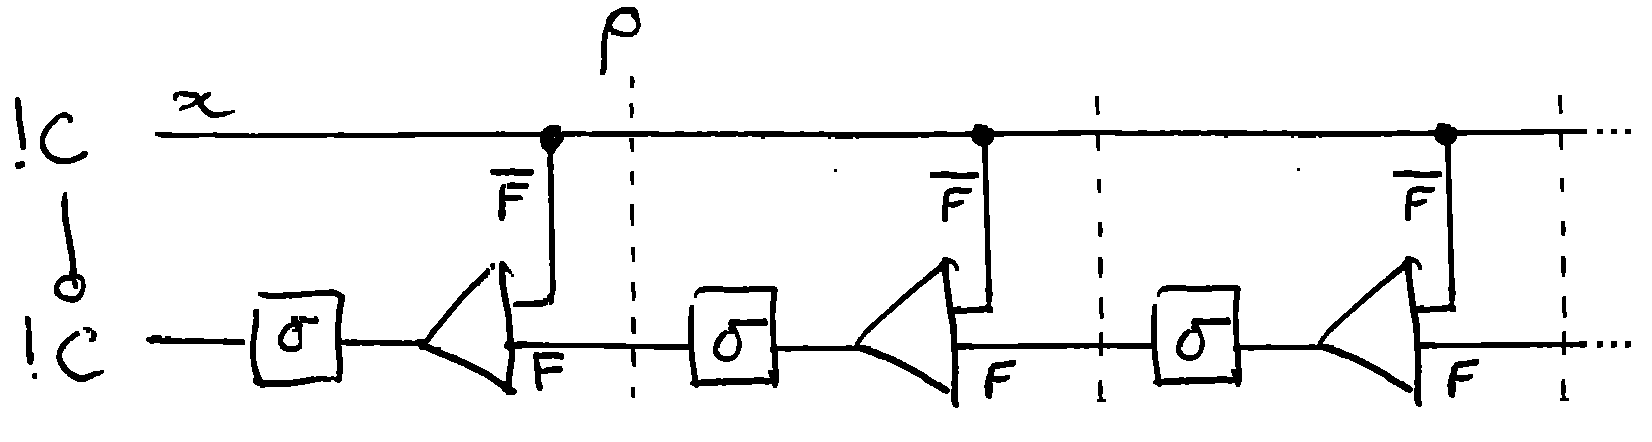
\includegraphics[scale=0.5]{linking-operator}
\end{center}

%}}}

\subsection{Semantics of Compcert languages} %{{{

%}}}

\subsection{External functions [?]} %{{{

[By which I mean the semantics of external functions
including memcpy, malloc, free \ldots
The semantics of those can be defined as strategies
and linked back.]

[One issue is:
Compcert's correctness theorem is
assuming that external functions behave in a certain way.
So if we remove them completely into an oracle
it won't be valid any more.
But,
we'd like to get rid of events completely,
so it'd ...]

%}}}

\subsection{Relation to operational semantics} %{{{

Oracle construction.

%}}}

\subsection{Properties} %{{{

Clight: Determined, innocent, well-bracketed. \\
Asm: Innocent, well-bracketed?

%}}}

%}}}

\newpage
\section{Kripke logical relations for Compcert} %{{{

%XXX: how does this relate to
%the intrinsic preorder in 3.5 of [Abramsky \emph{Game Semantics}]?
%Sound/complete reasoning principle?

\subsection{Overview} %{{{

In the broadest sense [/ ``In one interpretation''?],
\emph{logical relations} are structure-preserving relations,
in the same way that homomorphisms are structure-preserving maps
\citep{lrp}.
Given a set $W$ of \emph{possible worlds}
and an \emph{accessibility relation} $\leadsto$ on $W$,
a \emph{Kripke logical relation} is
a $W$-indexed family of logical relations $(R_w)_{w \in W}$.
These are not precise definitions;
for our purposes it will be sufficient
to define a notion of ``logical relation of $\mathcal{A}$s''
on a case-by-case basis,
for each structure $\mathcal{A}$ we consider.
The corresponding definition of a
``Kripke logical relation of $\mathcal{A}$s''
will follow.

\begin{example}[Kripke logical relaton of monoids]
A \emph{monoid} is a set $A$ equipped with
an associative binary operation $\cdot$ and
an identity element $\epsilon$.
A \emph{logical relation of monoids} between
a monoid $(A, \cdot_A, \epsilon_A)$ and
a monoid $(B, \cdot_B, \epsilon_B)$
is a relation $R \subseteq A \times B$
such that:
\begin{gather*}
u \ifr{R} u' \wedge v \ifr{R} v' \Rightarrow u \cdot_A v \ifr{R} u' \cdot_B v' \\
\epsilon_A \ifr{R} \epsilon_B
\end{gather*}
[Find good examples of monoids and a KLR between them.]
\end{example}

[Explain use in PL theory and role of KLR].

The simulation relations used by Compcert can be understood
as Kripke logical relations over
Compcert's operational semantics.
The relations between
the states and transition relations of \kw{Clight} or \kw{Asm}
are built up in a systematic way out of elementary relations
at basic types like \kw{mem} and \kw{val}.

For example,
Compcert's memory injections
define a Kripke logical relation \kw{inj} as follows.
The elementary relations \kw{Mem.inject} and \kw{Val.inject}
are indexed over the set of worlds \kw{meminj},
which specify how memory blocks in the source and target states
correspond to each other.
The accessibility relation \kw{inject\_incr}
specifies for a given injection
what are its possible ``futures'' are:
they should map existing blocks in the same way
but may additionally map blocks newly allocated in the source.
From \kw{Mem.inject}, \kw{Val.inject} and similary elementary relations,
more complex relations are defined,
culminating in a number of simulation diagrams.
Similarly,
\kw{Mem.extends}, \kw{Val.lessdef}, and related constructions
can be understood as the components of a KLR \kw{ext},
though one with a trivial set of worlds $\{*\}$.
Fig. X illustrates [much of Compcert's memory model spec
just expresses the compatibility of basic operations
with these KLRs and more].

In the following,
we generalize from \kw{inj} and \kw{ext} and
introduce a family of Kripke logical relations for Compcert,
which define logical relations at all the types
involved in Compcert's semantics.
These relations are compatible with
all appropriate elementary operations
(in particular, operations of the Compcert memory model).
They satisfy enough properties that
the \kw{Clight} and \kw{Asm} transition relations
are stable under any of them
(a relational parametricity theorem),
yet are flexible enough that encode many interesting properties,
giving us many theorems about Compcert's operational semantics
``for free''.

This reading of Compcert's foundations
in terms of logical relations
can provide us with new insight
[way to understand Compcert's complicated
statements about injections etc. in a uniform way]
[we will see also a guide for formulating our definitions
when moving into the realm of games].

%}}}

\subsection{Logical relations}

\subsection{Kripke relators}

Note that for a given Kripke frame $\langle W, \leadsto \rangle$,
a logical relation $R : \mathcal{R}(A, B)$
can be promoted to a $W$-indexed Kripke logical relation $\lceil R \rceil$
by simply ignoring the index so that $\lceil R \rceil_w = R$.
Likewise,
a relator
  $F : \mathcal{R}(A_1, B_1) \times \cdots \times \mathcal{R}(A_n, B_n) \rightarrow \mathcal{R}(A, B)$
can be promoted to its Kripke version
by pointwise extension over the set of possible worlds:
\begin{gather*}
  \lceil F \rceil : \mathcal{R}_W(A_1, B_1) \times \cdots \times \mathcal{R}_W(A_n, B_n) \rightarrow \mathcal{R}_W(A, B) \\
  \lceil F \rceil (R_1, \ldots, R_n)_w = F(R_{1,w}, \ldots, R_{n,w})
\end{gather*}
In addition,
$\Box, \Diamond : \mathcal{R}_W(A,B) \rightarrow \mathcal{R}_W(A,B)$
are the Kripke relators defined by:
\begin{align*}
  x \ifr{(\Box R)_w} y &\Leftrightarrow
    \forall w' \,.\, w \leadsto w' \rightarrow x \ifr{R_w} y \\
  x \ifr{(\Diamond R)_w} y &\Leftrightarrow
    \exists w' \,.\, w \leadsto w' \wedge x \ifr{R_w} y
\end{align*}

\begin{example}[Simulation diagram]
Consider a Kripke logical relation of sets $R : \mathcal{R}_W(A, B)$,
and two transition relations $\alpha : A \rightarrow \mathcal{P}(A)$
and $\beta : B \rightarrow \mathcal{P}(B)$.
The simulation diagram:
\[
  \begin{tikzcd}
    s_1 \arrow[r, "\alpha"]
        \arrow[d, dash, "R_w"'] &
    s_1' \arrow[d, dotted, dash, "R_{w'} \quad (w \leadsto w')"] \\
    s_2 \arrow[r, dotted, "\beta"] &
    s_2'
  \end{tikzcd}
\]
can be written as:
\[
  \alpha \ifr{R \rightarrow \mathcal{P}^+(\Diamond R)} \beta \,.
\]
\end{example}

\subsection{Basic types}

\paragraph{Pointers}

The Compcert memory model \cite{compcertmmv2}
represents the memory as a finite number of blocks,
each equipped with its own address space.
Block identifiers $b : \kw{block}$
are represented by positive integers,
and pointers specify an arbitrary offset within a given block:
\[
    \kw{ptr} = \kw{block} \times \mathbb{Z} \,.
\]
To keep our exposition concise and clear,
we will gloss over the technical details
associated with the encoding of offsets
as concrete binary integers,
and the associated modular arithmetic and overflow constraints.
In this setting,
a logical relation of Compcert pointers
is a relation $R \subseteq (\kw{block} \times \mathbb{Z}) \times (\kw{block} \times \mathbb{Z})$.
which satisfies the following \emph{shift-invariance} property:
\[
  \AxiomC{$(b_1, o_1) \ifr{R} (b_2, o_2)$}
  \UnaryInfC{$(b_1, o_1 + \delta) \ifr{R} (b_2, o_2 + \delta)$}
  \DisplayProof
\]
We write $R : \mathcal{R}(\kw{ptr})$.
Note that there is a one-to-one correspondance between
functional logical relations of pointers and
Compcert memory injections.

\paragraph{Values}

Next,
fix a logical relation of pointers $R^\kw{ptr} : \mathcal{R}(\kw{ptr})$
[XXX or set things up so that $R$ determines a unique pointer relation],
and consider Compcert's type \kw{val} of run-time values:
\[
  v : \kw{val} ::= \kw{Vundef}
          \alt \kw{Vint}(n)
          \alt \kw{Vlong}(n)
          \alt \kw{Vfloat}(x)
          \alt \kw{Vsingle}(x)
          \alt \kw{Vptr}(p)
\]
A logical relation of Compcert values
is a relation $R \subseteq \kw{val} \times \kw{val}$
which satisfies the following properties:
\begin{gather*}
  \kw{Vundef} \ifr{R} \kw{Vundef} \\
  \kw{Vint} \ifr{(=) \rightarrow R} \kw{Vint} \\
  \kw{Vlong} \ifr{(=) \rightarrow R} \kw{Vlong} \\
  \kw{Vfloat} \ifr{(=) \rightarrow R} \kw{Vfloat} \\
  \kw{Vsingle} \ifr{(=) \rightarrow R} \kw{Vsingle} \\
  \kw{Vptr} \ifr{R^\kw{ptr} \rightarrow R} \kw{Vptr}
\end{gather*}
[Add the other ones, note that it is determined by $(f, U^\kw{val}, U^\kw{ptr})$,
comment on the difficulties for composition.]

\paragraph{Memory states}



A Kripke logical relation of Compcert values 

\subsection{Simulation relation toolkits} %{{{

\begin{definition}[\kw{simrel}]
A Compcert \emph{simulation relation toolkit} $R$
is a tuple $(W_R, \leadsto_R, U^\kw{v}_R, U^\kw{b}_R, f_R, R^\kw{mem})$
such that:
\begin{itemize}
\item $(W_R, \leadsto_R)$
  is a preorder of $R$'s \emph{possible worlds};
\item $U^\kw{v}_R : \mathbb{B}$
  specifies whether undefined values on the left
  can be refined into non-pointer values on the right;
\item $U^\kw{b}_R : W_R \rightarrow \mathcal{P}(\kw{block})$
  specifies whether undefined values can be refined into pointers to a given block;
\item $f_R : W_R \rightarrow \kw{meminj}$
  specifies for each world how pointers should be related;
\item $R^\kw{mem} : W_R \rightarrow \mathcal{R}(\kw{mem})$
  specifies for each world how memory states should be related.
\end{itemize}
The components of $R$ must satisfy
a number of properties which are shown in Fig~\ref{fig:simrelprop}
and discussed below.
\end{definition}

\begin{figure}
  \small
  \[ R = (W, \leadsto, U^\kw{v}, U^\kw{b}, f, R^\kw{mem}) \]
  \noindent \fbox{$R_w^\kw{ptr}$} \hfill \ 
  \[
    \AxiomC{$f_w(b) = (b', \delta)$}
    \UnaryInfC{$(b, o) \ifr{R_w^\kw{ptr}} (b', o + \delta)$}
    \DisplayProof
  \]
  \noindent \fbox{$R^\kw{ptrbits}_w$} \hfill \ 
  \[
    \AxiomC{$f_w(b) = (b', \delta)$}
    \UnaryInfC{$(b, o) \ifr{R_w^\kw{ptrbits}} (b', \kw{Ptrofs.add}(o, \kw{Ptrofs.repr}(\delta)))$}
    \DisplayProof
  \]
  \noindent \fbox{$R_w^\kw{val}$} \hfill \ 
  \begin{align*}
    U^\kw{v} = \kw{t} &\Rightarrow
        \kw{Vundef} \ifr{R_w^\kw{val}} \kw{Vint}(n)
        \\
    U^\kw{v} = \kw{t} &\Rightarrow
        \kw{Vundef} \ifr{R_w^\kw{val}} \kw{Vlong}(n)
        \\
    U^\kw{v} = \kw{t} &\Rightarrow
        \kw{Vundef} \ifr{R_w^\kw{val}} \kw{Vfloat}(x)
        \\
    U^\kw{v} = \kw{t} &\Rightarrow
        \kw{Vundef} \ifr{R_w^\kw{val}} \kw{Vsingle}(x)
        \\
    U^\kw{b}_w(b_2) &\Rightarrow
        \kw{Vundef} \ifr{R_w^\kw{val}} \kw{Vptr}(b_2, o_2)
  \end{align*}
  \label{fig:simrel}
  \caption{Elementary relations associated with $R$}
\end{figure}

\begin{figure}
  \begin{gather*}
    U^\kw{b} \ifr{(\leadsto) \rightarrow (=) \rightarrow (\Rightarrow)} U^\kw{b} \\
    f \ifr{(\leadsto) \rightarrow \kw{inject\_incr}} f \\
    U^\kw{v} = \kw{t} \ \wedge\  p_1 \ifr{R^\kw{ptr}_w} (b_2, o_2) \ \Rightarrow\  U^\kw{b}_w(b_2) \\
    U^\kw{p}_w(b_2) \ \Rightarrow\  U^\kw{v} = \kw{t} \\
    [\ldots] \\
    \kw{Mem.alloc}
    \ifrw{R^\kw{mem} \rightarrow (=) \rightarrow (=) \rightarrow
      \Diamond (R^\kw{mem} \times R^\kw{block})}{w}
    \kw{Mem.alloc}
    \\
    \kw{Mem.free}
    \ifrw{R^\kw{mem} \rightarrow R^\kw{ptrrange} \rightarrow
      \kw{option}^+(\Diamond R^\kw{mem}))}{w}
    \kw{Mem.free}
    \\
    \ldots
  \end{gather*}
  \label{fig:simrelprop}
  \caption{Required properties for simulation relation toolkits}
\end{figure}

Simulation relation toolkits (\kw{simrel} for short)
are named this way because we will ultimately
use them to build simulation relations between
Compcert transition systems.

Values are related in a way that largely mirrors $\kw{Val.inject}\,f_w$,
however the additional parameters $U^\kw{v}$ and $U^\kw{b}$
specify whether $\kw{Vundef}$ should be allowed to refine defined values.
The ability to switch off this behavior of \kw{Val.inject} and \kw{Val.lessdef}
allows us to define the simulation relation toolkit \kw{id},
for which $R^\kw{mem}$ and $R^\kw{val}$ both reduce to equality,
as well as coreflexive \kw{simrel}s,
which can be used to encode a number of invariants.
The separate treatment of pointers with $U^\kw{b}$
is necessary when defining the composite \kw{simrel} $R_1 \circ R_2$.

Note that the relational property associated to $f$,
together with the definitions of
derived relations such as $R^\kw{ptr}$, $R^\kw{ptrbits}$, or $R^\kw{val}$,
ensure that these relations are monotonic in $w$,
in the sense that given $w \leadsto w'$,
it is possible to show that $R^x_w \subseteq R^x_{w'}$.
However,
this is not necessarily the case for $R^\kw{mem}$.



[Define inj, ext, id, $\circ$.]


Kripke logical relations of arenas, games, strategies.

It is in fact possible to define a
category of Compcert memory models and Compcert-compatible KLRs,
but for the work presented here we restrict our attention
to finite compositions of strong \textsf{ext} and \textsf{inj}.

%}}}

\subsection{Compcert's relational parametricity} %{{{

External call requirements expressed as KLR.

%}}}

\subsection{Game-theoretic simulations} %{{{

Compositional CompCert:
\begin{quote}
A deficiency of CompCert’s simulation proofs and of LSRs
was that they assumed conditions (1) and (2) at external calls,
but did not prove that these properties were preserved by compilation.
Directly imposing constraints (1) and (2)
onto the simulation clauses for internal steps does not work, however.
A compiled function should be allowed to
write to its own spill locations ---
just not to those of its caller.
\end{quote}
Go on to define massively complicated \emph{structured injections}.

But we don't need to!
Our KLR framework
mapped onto justification pointers
expresses just the right constraints!

%}}}

\subsection{Simulation reflection property} %{{{

Oracles and the simulation reflection property.

(Extensionality of function types.)

%}}}

%}}}

\newpage
\section{Compositional correctness of CompCertX} %{{{

%}}}

\newpage
\section{Linking with fancy contexts} %{{{

Show that we can link soundly with thread library, longjmp, cswitch, etc.

Verify some mixed C/asm program that uses this kind of assembly primitives.

\subsection{Long jumps}
\label{sec:longjmp}

The C standard library provides the following primitives
which implement ``non-local jumps'':
\begin{description}
\item[\texttt{setjmp(jmp\_buf env)}]
    saves the stack context into \texttt{env}
    and returns ...
\item[\texttt{longjmp(jmp\_buf env)}]
    interrupts normal control flow
    and restores the stack context previously saved in \texttt{env},
    causing the corresponding call to \texttt{setjmp}
    to return again,
    this time a non-zero value.
\end{description}
Because \kw{longjmp} triggers a control effect,
its semantics cannot be described
as that of a classical Compcert external function call.
However,
a version of \kw{setjmp} and \kw{longjmp}
can be modelled naturally as the strategy $\sigma_\kw{jmp}$
defined by the prefix closure of the following language:
\[
    \small
    \left(
    (\texttt{setjmp}()@m_i\ph{p1}\ \cdot\ \pt{p1}\underline{0@m_i})^* \ \cdot\ 
    \texttt{setjmp}()@m\ph{p} \ \cdot\ \pt{p}\underline{0@m}\ \cdot\ 
    \texttt{longjmp}()@m'\ \cdot\ \pt{p}\underline{1@m'}
    \right)^*
\]

%}}}

\newpage
\section{Related Work} %{{{

Interaction semantics is an automaton formulation of $EC \Rightarrow EC$
(follows Ghica 2012),
but our semantic domain more open-ended and
we can use Compcert with fancier games
(say event traces etc).
Also,
by oversimplifying they've given up the structure
that allows us to define our magical KLRs
and they have to put it back in,
in a much more contrived and ad-hoc way.
(Also by mixing internal steps and interaction steps per Ghica 2012.)

%}}}

\newpage
\section{Future work} %{{{

Simulation among different games,
also $\sigma^+ \le \tau^+$.

%}}}

\bibliography{lwcc}

\end{document}
